\documentclass[tikz,border=10pt]{standalone}
\usetikzlibrary{positioning, backgrounds, calc}

\begin{document}
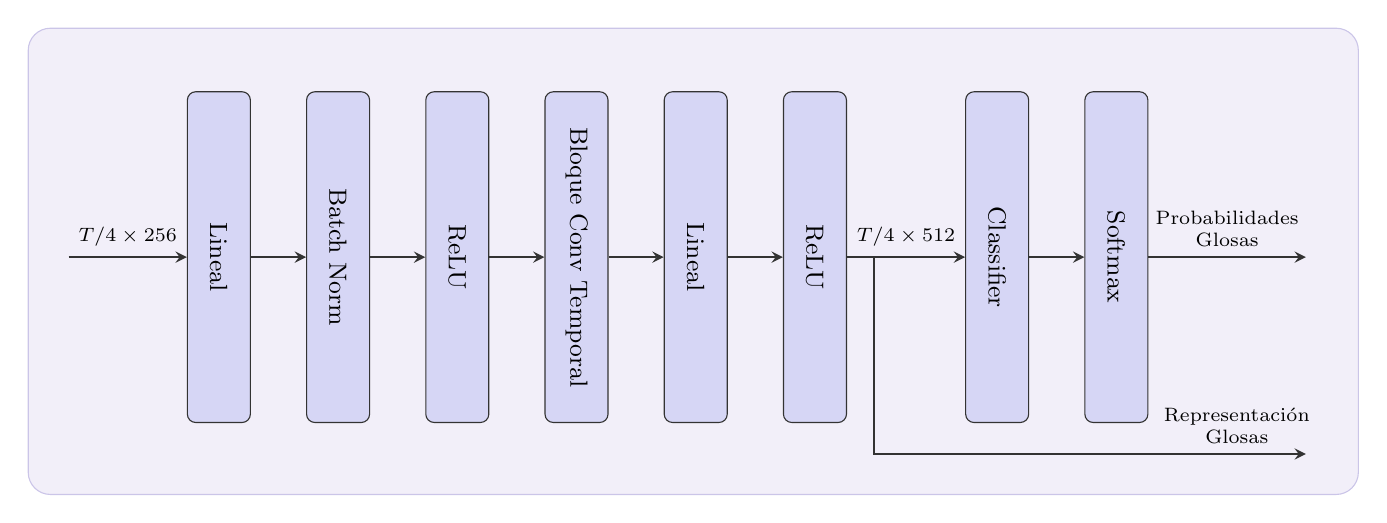
\begin{tikzpicture}[
    node distance=0.7cm,
    % Estilo idéntico a la imagen proporcionada: bloques grises, bordes negros, texto rotado
    vnode/.style={
        rectangle,
        draw=black!80,
        fill=blue!60!gray!20,
        rounded corners=3pt,
        minimum height=4.2cm,
        minimum width=0.8cm,
        align=center,
        font=\small
    },
    arr/.style={->, >=stealth, thick, draw=black!80}
]

    % --- ENTRADA ---
    \coordinate (in);

    % --- NODOS DE LA RED DE CABECERA ---
    %\node[vnode, right=1cm of in] (pool) {\rotatebox{-90}{Spatial Pooling}};
    \node[vnode, right=1.5cm of in] (lin1) {\rotatebox{-90}{Lineal}};
    \node[vnode, right=of lin1] (bn) {\rotatebox{-90}{Batch Norm}};
    \node[vnode, right=of bn] (relu1) {\rotatebox{-90}{ReLU}};

    % Agrupado como bloque para mantener estética
    \node[vnode, right=of relu1] (tconv) {\rotatebox{-90}{Bloque Conv Temporal}};

    \node[vnode, right=of tconv] (lin2) {\rotatebox{-90}{Lineal}};
    \node[vnode, right=of lin2] (relu2) {\rotatebox{-90}{ReLU}};

    % Separación extra para denotar la representación final antes de clasificar
    \node[vnode, right=1.5cm of relu2] (clf) {\rotatebox{-90}{Classifier}};
    \node[vnode, right=of clf] (soft) {\rotatebox{-90}{Softmax}};

    % --- SALIDA ---
    \coordinate[right=2cm of soft] (out);

    \coordinate[below=2.5cm of out] (out2);

    % --- CONEXIONES Y DIMENSIONES (TEXTO MATEMÁTICO SOBRE LAS FLECHAS) ---
    %\draw[arr] (in) -- (lin1);
    \draw[arr] (in) -- node[above, font=\scriptsize] {$T/4 \times 256$} (lin1);
    \draw[arr] (lin1) -- (bn);
    \draw[arr] (bn) -- (relu1);
    \draw[arr] (relu1) -- (tconv);
    \draw[arr] (tconv) -- (lin2);
    \draw[arr] (lin2) -- (relu2);

    % La salida de aquí es la "Representación de la glosa"
    \draw[arr] (relu2) -- node[above, font=\scriptsize] {$T/4 \times 512$} (clf);
    \draw[arr] (clf) -- (soft);
    \draw[arr] (soft) -- node[above, font=\scriptsize, align=center] {Probabilidades\\Glosas} (out);

    \draw[arr] (relu2) -- ++(0.75,0)  |-  node[pos=0.92, above, font=\scriptsize, align=center] {Representación\\Glosas} (out2); %
    % --- FONDO AZUL CLARO ESTILO "IMAGE_AF9328.PNG" ---
    \begin{scope}[on background layer]
        \path[draw=cyan!10!blue!20, fill=cyan!5!blue!5, rounded corners=8pt]
        ([xshift=-0.5cm, yshift=0.8cm]current bounding box.north west)
        rectangle ([xshift=0.5cm, yshift=-0.5cm]current bounding box.south east);
    \end{scope}

\end{tikzpicture}
\end{document}
